\chapter{Osnove grafova}

Mnogi se programski zadaci mogu riješiti tako da
zadatak modeliramo kao problem na grafu
i primijenimo prikladan algoritam na grafovima.
Tipičan primjer grafa je mreža
cesta i gradova u nekoj državi.
Ponekad je, međutim, graf skriven
u zadatku pa ga može biti teško prepoznati.

Ovaj dio knjige obrađuje algoritme na grafovima,
s posebnim naglaskom na teme koje
su važne u natjecateljskom programiranju.
U ovom poglavlju proći ćemo kroz pojmove
povezane s grafovima
i proučiti različite načine prikaza grafova u algoritmima.

\section{Terminologija grafova}

\index{graf}
\index{čvor}
\index{brid}

\key{Graf} se sastoji od \key{čvorova}
i \key{bridova}. U ovoj knjizi
varijabla $n$ označava broj čvorova
u grafu, a varijabla $m$ označava
broj bridova.
Čvorovi su numerirani
cijelim brojevima $1,2,\ldots,n$.

Na primjer, sljedeći graf sastoji se od 5 čvorova i 7 bridova:

\begin{center}
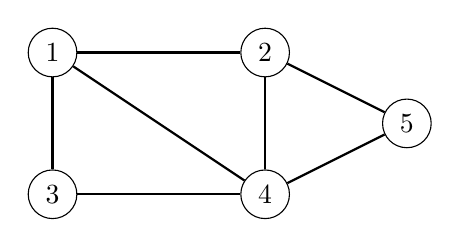
\begin{tikzpicture}[scale=0.9]
\node[draw, circle] (1) at (1,3) {$1$};
\node[draw, circle] (2) at (4,3) {$2$};
\node[draw, circle] (3) at (1,1) {$3$};
\node[draw, circle] (4) at (4,1) {$4$};
\node[draw, circle] (5) at (6,2) {$5$};

\path[draw,thick,-] (1) -- (2);
\path[draw,thick,-] (1) -- (3);
\path[draw,thick,-] (1) -- (4);
\path[draw,thick,-] (3) -- (4);
\path[draw,thick,-] (2) -- (4);
\path[draw,thick,-] (2) -- (5);
\path[draw,thick,-] (4) -- (5);
\end{tikzpicture}
\end{center}

\index{put}

\key{Put} vodi od čvora $a$ do čvora $b$
kroz bridove grafa.
\key{Dužina} puta je broj
bridova na njemu.
Na primjer, gornji graf sadrži
put $1 \rightarrow 3 \rightarrow 4 \rightarrow 5$
dužine 3
od čvora 1 do čvora 5:

\begin{center}
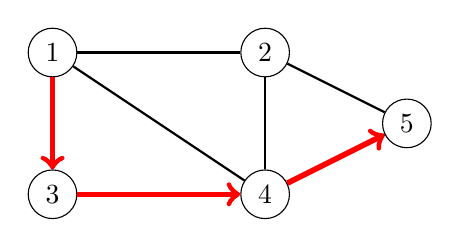
\begin{tikzpicture}[scale=0.9]
\node[draw, circle] (1) at (1,3) {$1$};
\node[draw, circle] (2) at (4,3) {$2$};
\node[draw, circle] (3) at (1,1) {$3$};
\node[draw, circle] (4) at (4,1) {$4$};
\node[draw, circle] (5) at (6,2) {$5$};

\path[draw,thick,-] (1) -- (2);
\path[draw,thick,-] (1) -- (3);
\path[draw,thick,-] (1) -- (4);
\path[draw,thick,-] (3) -- (4);
\path[draw,thick,-] (2) -- (4);
\path[draw,thick,-] (2) -- (5);
\path[draw,thick,-] (4) -- (5);

\path[draw=red,thick,->,line width=2pt] (1) -- (3);
\path[draw=red,thick,->,line width=2pt] (3) -- (4);
\path[draw=red,thick,->,line width=2pt] (4) -- (5);
\end{tikzpicture}
\end{center}

\index{ciklus}

Put je \key{ciklus} ako su prvi i posljednji
čvor jednaki.
Na primjer, gornji graf sadrži
ciklus $1 \rightarrow 3 \rightarrow 4 \rightarrow 1$.
Put je \key{jednostavan} ako se svaki čvor pojavljuje
najviše jednom na putu.


% 
% \begin{itemize}
% \item $1 \rightarrow 2 \rightarrow 5$ (dužina 2)
% \item $1 \rightarrow 4 \rightarrow 5$ (dužina 2)
% \item $1 \rightarrow 2 \rightarrow 4 \rightarrow 5$ (dužina 3)
% \item $1 \rightarrow 3 \rightarrow 4 \rightarrow 5$ (dužina 3)
% \item $1 \rightarrow 4 \rightarrow 2 \rightarrow 5$ (dužina 3)
% \item $1 \rightarrow 3 \rightarrow 4 \rightarrow 2 \rightarrow 5$ (dužina 4)
% \end{itemize}

\subsubsection{Povezanost}

\index{povezan graf}

Graf je \key{povezan} ako postoji put
između bilo koja dva čvora.
Na primjer, sljedeći graf je povezan:
\begin{center}
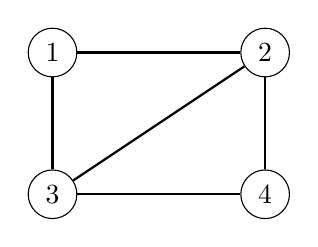
\begin{tikzpicture}[scale=0.9]
\node[draw, circle] (1) at (1,3) {$1$};
\node[draw, circle] (2) at (4,3) {$2$};
\node[draw, circle] (3) at (1,1) {$3$};
\node[draw, circle] (4) at (4,1) {$4$};
\path[draw,thick,-] (1) -- (2);
\path[draw,thick,-] (1) -- (3);
\path[draw,thick,-] (2) -- (3);
\path[draw,thick,-] (3) -- (4);
\path[draw,thick,-] (2) -- (4);
\end{tikzpicture}
\end{center}

Sljedeći graf nije povezan,
jer nije moguće doći
od čvora 4 do bilo kojeg drugog čvora:
\begin{center}
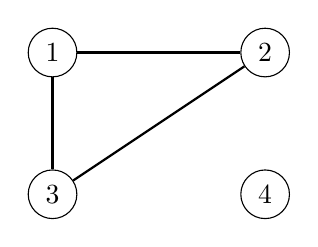
\begin{tikzpicture}[scale=0.9]
\node[draw, circle] (1) at (1,3) {$1$};
\node[draw, circle] (2) at (4,3) {$2$};
\node[draw, circle] (3) at (1,1) {$3$};
\node[draw, circle] (4) at (4,1) {$4$};
\path[draw,thick,-] (1) -- (2);
\path[draw,thick,-] (1) -- (3);
\path[draw,thick,-] (2) -- (3);
\end{tikzpicture}
\end{center}

\index{komponenta}

Povezani dijelovi grafa
nazivaju se njegove \key{komponente}.
Na primjer, sljedeći graf
sadrži tri komponente:
$\{1,\,2,\,3\}$,
$\{4,\,5,\,6,\,7\}$ i
$\{8\}$.
\begin{center}
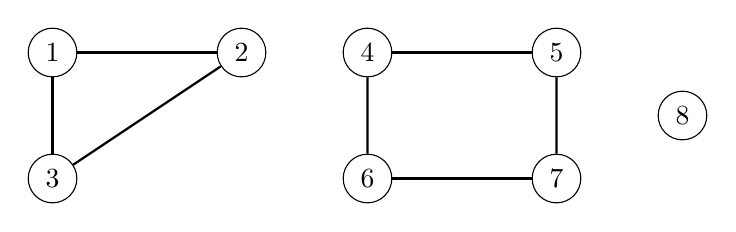
\begin{tikzpicture}[scale=0.8]
\node[draw, circle] (1) at (1,3) {$1$};
\node[draw, circle] (2) at (4,3) {$2$};
\node[draw, circle] (3) at (1,1) {$3$};

\node[draw, circle] (6) at (6,1) {$6$};
\node[draw, circle] (7) at (9,1) {$7$};
\node[draw, circle] (4) at (6,3) {$4$};
\node[draw, circle] (5) at (9,3) {$5$};

\node[draw, circle] (8) at (11,2) {$8$};

\path[draw,thick,-] (1) -- (2);
\path[draw,thick,-] (2) -- (3);
\path[draw,thick,-] (1) -- (3);
\path[draw,thick,-] (4) -- (5);
\path[draw,thick,-] (5) -- (7);
\path[draw,thick,-] (6) -- (7);
\path[draw,thick,-] (6) -- (4);
\end{tikzpicture}
\end{center}

\index{stablo}

\key{Stablo} je povezan graf
koji se sastoji od $n$ čvorova i $n-1$ bridova.
Između bilo koja dva čvora stabla
postoji jedinstven put.
Na primjer, sljedeći graf je stablo:

\begin{center}
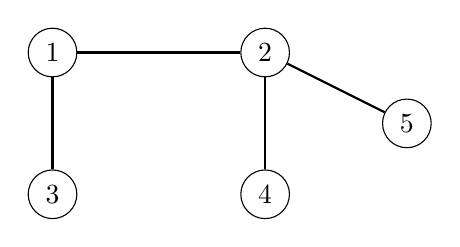
\begin{tikzpicture}[scale=0.9]
\node[draw, circle] (1) at (1,3) {$1$};
\node[draw, circle] (2) at (4,3) {$2$};
\node[draw, circle] (3) at (1,1) {$3$};
\node[draw, circle] (4) at (4,1) {$4$};
\node[draw, circle] (5) at (6,2) {$5$};

\path[draw,thick,-] (1) -- (2);
\path[draw,thick,-] (1) -- (3);
%\path[draw,thick,-] (1) -- (4);
\path[draw,thick,-] (2) -- (5);
\path[draw,thick,-] (2) -- (4);
%\path[draw,thick,-] (4) -- (5);
\end{tikzpicture}
\end{center}

\subsubsection{Smjerovi bridova}

\index{usmjereni graf}

Graf je \key{usmjeren}
ako se bridovima može prolaziti
samo u jednom smjeru.
Na primjer, sljedeći graf je usmjeren:
\begin{center}
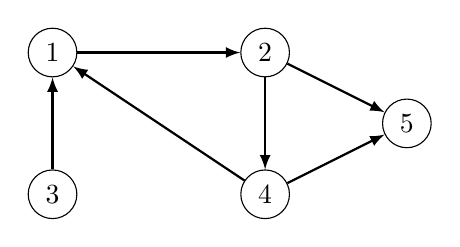
\begin{tikzpicture}[scale=0.9]
\node[draw, circle] (1) at (1,3) {$1$};
\node[draw, circle] (2) at (4,3) {$2$};
\node[draw, circle] (3) at (1,1) {$3$};
\node[draw, circle] (4) at (4,1) {$4$};
\node[draw, circle] (5) at (6,2) {$5$};
\path[draw,thick,->,>=latex] (1) -- (2);
\path[draw,thick,->,>=latex] (2) -- (4);
\path[draw,thick,->,>=latex] (2) -- (5);
\path[draw,thick,->,>=latex] (4) -- (5);
\path[draw,thick,->,>=latex] (4) -- (1);
\path[draw,thick,->,>=latex] (3) -- (1);
\end{tikzpicture}
\end{center}

Gornji graf sadrži
put $3 \rightarrow 1 \rightarrow 2 \rightarrow 5$
od čvora $3$ do čvora $5$,
ali ne postoji put od čvora $5$ do čvora $3$.

\subsubsection{Težine bridova}

\index{težinski graf}

U \key{težinskom} grafu svakom je bridu dodijeljena
\key{težina}.
Težine se često interpretiraju kao dužine bridova.
Na primjer, sljedeći graf je težinski:
\begin{center}
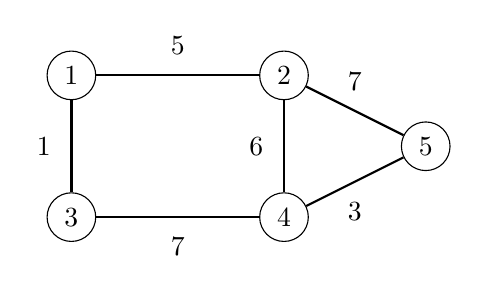
\begin{tikzpicture}[scale=0.9]
\node[draw, circle] (1) at (1,3) {$1$};
\node[draw, circle] (2) at (4,3) {$2$};
\node[draw, circle] (3) at (1,1) {$3$};
\node[draw, circle] (4) at (4,1) {$4$};
\node[draw, circle] (5) at (6,2) {$5$};
\path[draw,thick,-] (1) -- node[font=\small,label=above:5] {} (2);
\path[draw,thick,-] (1) -- node[font=\small,label=left:1] {} (3);
\path[draw,thick,-] (3) -- node[font=\small,label=below:7] {} (4);
\path[draw,thick,-] (2) -- node[font=\small,label=left:6] {} (4);
\path[draw,thick,-] (2) -- node[font=\small,label=above:7] {} (5);
\path[draw,thick,-] (4) -- node[font=\small,label=below:3] {} (5);
\end{tikzpicture}
\end{center}

Dužina puta u težinskom grafu
je suma težina bridova na tom putu.
Na primjer, u gornjem grafu
dužina puta
$1 \rightarrow 2 \rightarrow 5$ iznosi $12$,
a dužina puta
$1 \rightarrow 3 \rightarrow 4 \rightarrow 5$ iznosi $11$.
Drugi navedeni put je \key{najkraći} put od čvora $1$ do čvora $5$.

\subsubsection{Susjedi i stupnjevi}

\index{susjed}
\index{stupanj}

Dva su čvora \key{susjedi} ili \key{susjedni}
ako između njih postoji brid.
\key{Stupanj} čvora
je broj njegovih susjeda.
Na primjer, u sljedećem grafu
susjedi čvora 2 su 1, 4 i 5,
pa je njegov stupanj 3.

\begin{center}
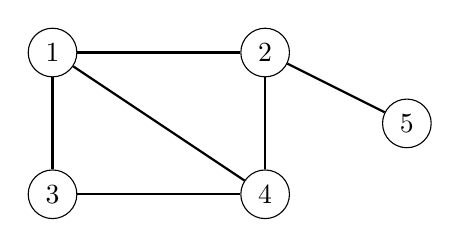
\begin{tikzpicture}[scale=0.9]
\node[draw, circle] (1) at (1,3) {$1$};
\node[draw, circle] (2) at (4,3) {$2$};
\node[draw, circle] (3) at (1,1) {$3$};
\node[draw, circle] (4) at (4,1) {$4$};
\node[draw, circle] (5) at (6,2) {$5$};

\path[draw,thick,-] (1) -- (2);
\path[draw,thick,-] (1) -- (3);
\path[draw,thick,-] (1) -- (4);
\path[draw,thick,-] (3) -- (4);
\path[draw,thick,-] (2) -- (4);
\path[draw,thick,-] (2) -- (5);
%\path[draw,thick,-] (4) -- (5);
\end{tikzpicture}
\end{center}

Suma stupnjeva u grafu uvijek je $2m$,
gdje je $m$ broj bridova,
jer svaki brid
povećava stupanj točno dvaju čvorova za jedan.
Zbog toga je suma stupnjeva uvijek parna.

\index{regularni graf}
\index{potpuni graf}

Graf je \key{regularan} ako je
stupanj svakog čvora konstanta $d$.
Graf je \key{potpun} ako je
stupanj svakog čvora $n-1$, tj.
graf sadrži sve moguće bridove
između čvorova.

\index{ulazni stupanj}
\index{izlazni stupanj}

U usmjerenom grafu \key{ulazni stupanj}
čvora je broj bridova
koji završavaju u tom čvoru,
a \key{izlazni stupanj} čvora
je broj bridova koji počinju u tom čvoru.
Na primjer, u sljedećem grafu
ulazni stupanj čvora 2 je 2,
a izlazni stupanj čvora 2 je 1.

\begin{center}
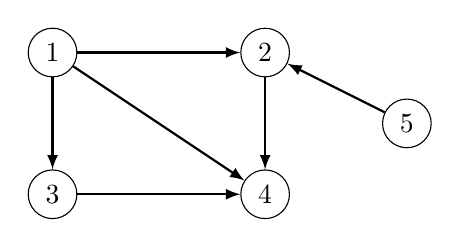
\begin{tikzpicture}[scale=0.9]
\node[draw, circle] (1) at (1,3) {$1$};
\node[draw, circle] (2) at (4,3) {$2$};
\node[draw, circle] (3) at (1,1) {$3$};
\node[draw, circle] (4) at (4,1) {$4$};
\node[draw, circle] (5) at (6,2) {$5$};

\path[draw,thick,->,>=latex] (1) -- (2);
\path[draw,thick,->,>=latex] (1) -- (3);
\path[draw,thick,->,>=latex] (1) -- (4);
\path[draw,thick,->,>=latex] (3) -- (4);
\path[draw,thick,->,>=latex] (2) -- (4);
\path[draw,thick,<-,>=latex] (2) -- (5);
\end{tikzpicture}
\end{center}

\subsubsection{Bojanja}

\index{bojanje}
\index{bipartitni graf}

U \key{bojanju} grafa
svakom je čvoru dodijeljena boja tako da
nikoja dva susjedna čvora nemaju istu boju.

Graf je \key{bipartitan} ako
ga je moguće obojiti pomoću dvije boje.
Pokazuje se da je graf bipartitan
točno onda kada ne sadrži ciklus
s neparnim brojem bridova.
Na primjer, graf
\begin{center}
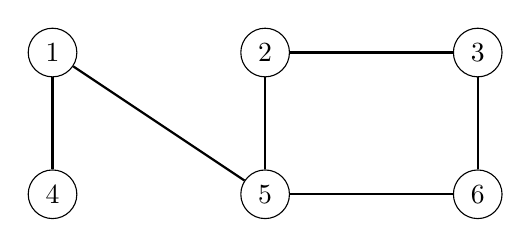
\begin{tikzpicture}[scale=0.9]
\node[draw, circle] (1) at (1,3) {$2$};
\node[draw, circle] (2) at (4,3) {$3$};
\node[draw, circle] (3) at (1,1) {$5$};
\node[draw, circle] (4) at (4,1) {$6$};
\node[draw, circle] (5) at (-2,1) {$4$};
\node[draw, circle] (6) at (-2,3) {$1$};
\path[draw,thick,-] (1) -- (2);
\path[draw,thick,-] (1) -- (3);
\path[draw,thick,-] (3) -- (4);
\path[draw,thick,-] (2) -- (4);
\path[draw,thick,-] (3) -- (6);
\path[draw,thick,-] (5) -- (6);
\end{tikzpicture}
\end{center}
je bipartitan, jer ga možemo obojiti na sljedeći način:
\begin{center}
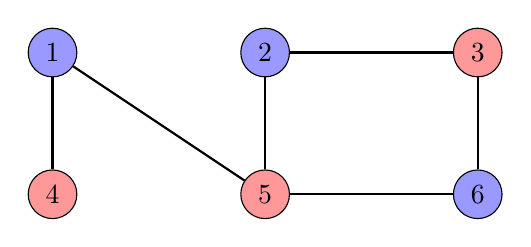
\begin{tikzpicture}[scale=0.9]
\node[draw, circle, fill=blue!40] (1) at (1,3) {$2$};
\node[draw, circle, fill=red!40] (2) at (4,3) {$3$};
\node[draw, circle, fill=red!40] (3) at (1,1) {$5$};
\node[draw, circle, fill=blue!40] (4) at (4,1) {$6$};
\node[draw, circle, fill=red!40] (5) at (-2,1) {$4$};
\node[draw, circle, fill=blue!40] (6) at (-2,3) {$1$};
\path[draw,thick,-] (1) -- (2);
\path[draw,thick,-] (1) -- (3);
\path[draw,thick,-] (3) -- (4);
\path[draw,thick,-] (2) -- (4);
\path[draw,thick,-] (3) -- (6);
\path[draw,thick,-] (5) -- (6);
\end{tikzpicture}
\end{center}
Međutim, graf
\begin{center}
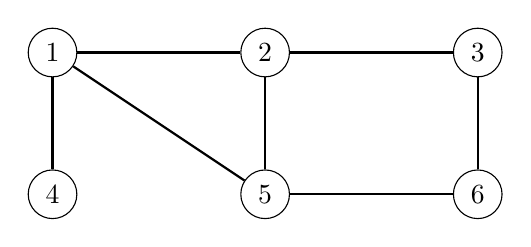
\begin{tikzpicture}[scale=0.9]
\node[draw, circle] (1) at (1,3) {$2$};
\node[draw, circle] (2) at (4,3) {$3$};
\node[draw, circle] (3) at (1,1) {$5$};
\node[draw, circle] (4) at (4,1) {$6$};
\node[draw, circle] (5) at (-2,1) {$4$};
\node[draw, circle] (6) at (-2,3) {$1$};
\path[draw,thick,-] (1) -- (2);
\path[draw,thick,-] (1) -- (3);
\path[draw,thick,-] (3) -- (4);
\path[draw,thick,-] (2) -- (4);
\path[draw,thick,-] (3) -- (6);
\path[draw,thick,-] (5) -- (6);
\path[draw,thick,-] (1) -- (6);
\end{tikzpicture}
\end{center}
nije bipartitan, jer nije moguće obojiti
sljedeći ciklus od tri čvora pomoću dvije boje:
\begin{center}
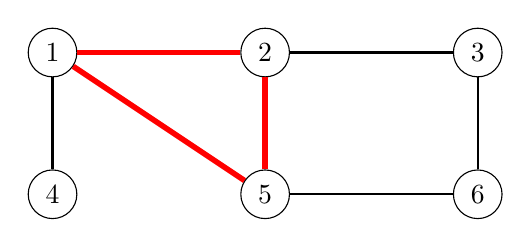
\begin{tikzpicture}[scale=0.9]
\node[draw, circle] (1) at (1,3) {$2$};
\node[draw, circle] (2) at (4,3) {$3$};
\node[draw, circle] (3) at (1,1) {$5$};
\node[draw, circle] (4) at (4,1) {$6$};
\node[draw, circle] (5) at (-2,1) {$4$};
\node[draw, circle] (6) at (-2,3) {$1$};
\path[draw,thick,-] (1) -- (2);
\path[draw,thick,-] (1) -- (3);
\path[draw,thick,-] (3) -- (4);
\path[draw,thick,-] (2) -- (4);
\path[draw,thick,-] (3) -- (6);
\path[draw,thick,-] (5) -- (6);
\path[draw,thick,-] (1) -- (6);

\path[draw=red,thick,-,line width=2pt] (1) -- (3);
\path[draw=red,thick,-,line width=2pt] (3) -- (6);
\path[draw=red,thick,-,line width=2pt] (6) -- (1);
\end{tikzpicture}
\end{center}

\subsubsection{Jednostavnost}

\index{jednostavan graf}

Graf je \key{jednostavan}
ako nijedan brid ne počinje i ne završava u istom čvoru
te ako između dvaju čvorova ne postoji
više bridova.
Često pretpostavljamo da su grafovi jednostavni.
Na primjer, sljedeći graf \emph{nije} jednostavan:
\begin{center}
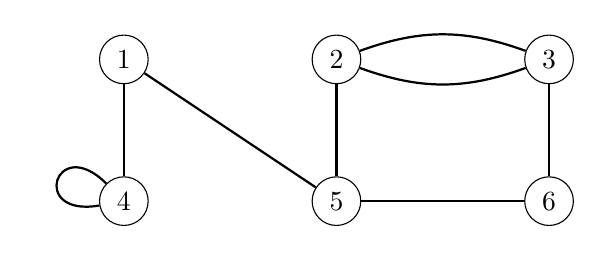
\begin{tikzpicture}[scale=0.9]
\node[draw, circle] (1) at (1,3) {$2$};
\node[draw, circle] (2) at (4,3) {$3$};
\node[draw, circle] (3) at (1,1) {$5$};
\node[draw, circle] (4) at (4,1) {$6$};
\node[draw, circle] (5) at (-2,1) {$4$};
\node[draw, circle] (6) at (-2,3) {$1$};

\path[draw,thick,-] (1) edge [bend right=20] (2);
\path[draw,thick,-] (2) edge [bend right=20] (1);
%\path[draw,thick,-] (1) -- (2);
\path[draw,thick,-] (1) -- (3);
\path[draw,thick,-] (3) -- (4);
\path[draw,thick,-] (2) -- (4);
\path[draw,thick,-] (3) -- (6);
\path[draw,thick,-] (5) -- (6);

\tikzset{every loop/.style={in=135,out=190}}
\path[draw,thick,-] (5) edge [loop left] (5);
\end{tikzpicture}
\end{center}

\section{Prikaz grafa}

Postoji nekoliko načina prikaza grafova
u algoritmima.
Odabir strukture podataka
ovisi o veličini grafa i
o načinu na koji ga algoritam obrađuje.
Dalje ćemo proći kroz tri uobičajena prikaza.

\subsubsection{Prikaz listama susjedstva}

\index{lista susjedstva}

U prikazu listama susjedstva
svakom je čvoru $x$ u grafu dodijeljena \key{lista susjedstva}
koja se sastoji od čvorova
do kojih iz $x$ postoji brid.
Liste susjedstva najpopularniji su
način prikaza grafova i većina se algoritama može
efikasno implementirati pomoću njih.

Praktičan način pohrane listi susjedstva je deklaracija
niza vektora na sljedeći način:
\begin{lstlisting}
vector<int> adj[N];
\end{lstlisting}

Konstanta $N$ odabire se tako da se sve
liste susjedstva mogu pohraniti.
Na primjer, graf

\begin{center}
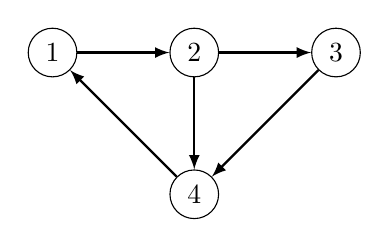
\begin{tikzpicture}[scale=0.9]
\node[draw, circle] (1) at (1,3) {$1$};
\node[draw, circle] (2) at (3,3) {$2$};
\node[draw, circle] (3) at (5,3) {$3$};
\node[draw, circle] (4) at (3,1) {$4$};

\path[draw,thick,->,>=latex] (1) -- (2);
\path[draw,thick,->,>=latex] (2) -- (3);
\path[draw,thick,->,>=latex] (2) -- (4);
\path[draw,thick,->,>=latex] (3) -- (4);
\path[draw,thick,->,>=latex] (4) -- (1);
\end{tikzpicture}
\end{center}
može se pohraniti na sljedeći način:
\begin{lstlisting}
adj[1].push_back(2);
adj[2].push_back(3);
adj[2].push_back(4);
adj[3].push_back(4);
adj[4].push_back(1);
\end{lstlisting}

Ako je graf neusmjeren, može se pohraniti na sličan način,
ali se svaki brid dodaje u oba smjera.

Za težinski graf struktura se može proširiti
na sljedeći način:

\begin{lstlisting}
vector<pair<int,int>> adj[N];
\end{lstlisting}

U tom slučaju lista susjedstva čvora $a$
sadrži par $(b,w)$
uvijek kada postoji brid od čvora $a$ do čvora $b$
s težinom $w$. Na primjer, graf

\begin{center}
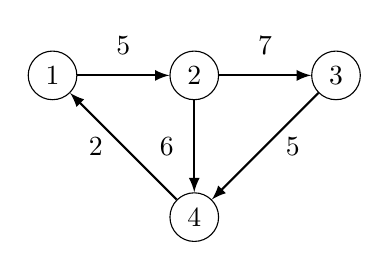
\begin{tikzpicture}[scale=0.9]
\node[draw, circle] (1) at (1,3) {$1$};
\node[draw, circle] (2) at (3,3) {$2$};
\node[draw, circle] (3) at (5,3) {$3$};
\node[draw, circle] (4) at (3,1) {$4$};

\path[draw,thick,->,>=latex] (1) -- node[font=\small,label=above:5] {} (2);
\path[draw,thick,->,>=latex] (2) -- node[font=\small,label=above:7] {} (3);
\path[draw,thick,->,>=latex] (2) -- node[font=\small,label=left:6] {} (4);
\path[draw,thick,->,>=latex] (3) -- node[font=\small,label=right:5] {} (4);
\path[draw,thick,->,>=latex] (4) -- node[font=\small,label=left:2] {} (1);
\end{tikzpicture}
\end{center}
može se pohraniti na sljedeći način:
\begin{lstlisting}
adj[1].push_back({2,5});
adj[2].push_back({3,7});
adj[2].push_back({4,6});
adj[3].push_back({4,5});
adj[4].push_back({1,2});
\end{lstlisting}

Prednost korištenja listi susjedstva je što
možemo efikasno naći čvorove u koje
se iz danog čvora možemo pomaknuti preko brida.
Na primjer, sljedeća petlja prolazi kroz sve čvorove
u koje se možemo pomaknuti iz čvora $s$:

\begin{lstlisting}
for (auto u : adj[s]) {
    // process node u
}
\end{lstlisting}

\subsubsection{Prikaz matricom susjedstva}

\index{matrica susjedstva}

\key{Matrica susjedstva} je dvodimenzionalni niz
koji pokazuje koje bridove graf sadrži.
Iz matrice susjedstva možemo efikasno provjeriti
postoji li brid između dvaju čvorova.
Matrica se može pohraniti kao niz
\begin{lstlisting}
int adj[N][N];
\end{lstlisting}
gdje svaka vrijednost $\texttt{adj}[a][b]$ pokazuje
sadrži li graf brid od
čvora $a$ do čvora $b$.
Ako je brid uključen u graf,
tada je $\texttt{adj}[a][b]=1$,
a inače je $\texttt{adj}[a][b]=0$.
Na primjer, graf
\begin{center}
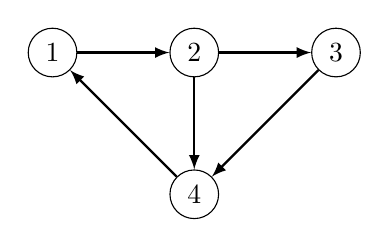
\begin{tikzpicture}[scale=0.9]
\node[draw, circle] (1) at (1,3) {$1$};
\node[draw, circle] (2) at (3,3) {$2$};
\node[draw, circle] (3) at (5,3) {$3$};
\node[draw, circle] (4) at (3,1) {$4$};

\path[draw,thick,->,>=latex] (1) -- (2);
\path[draw,thick,->,>=latex] (2) -- (3);
\path[draw,thick,->,>=latex] (2) -- (4);
\path[draw,thick,->,>=latex] (3) -- (4);
\path[draw,thick,->,>=latex] (4) -- (1);
\end{tikzpicture}
\end{center}
može se prikazati na sljedeći način:
\begin{center}
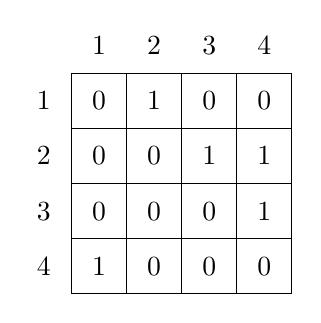
\begin{tikzpicture}[scale=0.7]
\draw (0,0) grid (4,4);
\node at (0.5,0.5) {1};
\node at (1.5,0.5) {0};
\node at (2.5,0.5) {0};
\node at (3.5,0.5) {0};
\node at (0.5,1.5) {0};
\node at (1.5,1.5) {0};
\node at (2.5,1.5) {0};
\node at (3.5,1.5) {1};
\node at (0.5,2.5) {0};
\node at (1.5,2.5) {0};
\node at (2.5,2.5) {1};
\node at (3.5,2.5) {1};
\node at (0.5,3.5) {0};
\node at (1.5,3.5) {1};
\node at (2.5,3.5) {0};
\node at (3.5,3.5) {0};
\node at (-0.5,0.5) {4};
\node at (-0.5,1.5) {3};
\node at (-0.5,2.5) {2};
\node at (-0.5,3.5) {1};
\node at (0.5,4.5) {1};
\node at (1.5,4.5) {2};
\node at (2.5,4.5) {3};
\node at (3.5,4.5) {4};
\end{tikzpicture}
\end{center}

Ako je graf težinski, prikaz matricom
susjedstva može se proširiti tako da
matrica sadrži težinu brida
ako brid postoji.
Uz takav prikaz, graf

\begin{center}
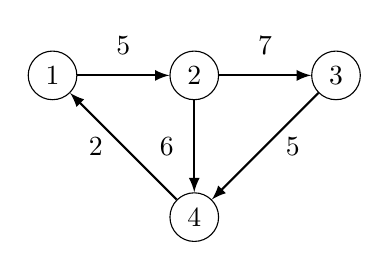
\begin{tikzpicture}[scale=0.9]
\node[draw, circle] (1) at (1,3) {$1$};
\node[draw, circle] (2) at (3,3) {$2$};
\node[draw, circle] (3) at (5,3) {$3$};
\node[draw, circle] (4) at (3,1) {$4$};

\path[draw,thick,->,>=latex] (1) -- node[font=\small,label=above:5] {} (2);
\path[draw,thick,->,>=latex] (2) -- node[font=\small,label=above:7] {} (3);
\path[draw,thick,->,>=latex] (2) -- node[font=\small,label=left:6] {} (4);
\path[draw,thick,->,>=latex] (3) -- node[font=\small,label=right:5] {} (4);
\path[draw,thick,->,>=latex] (4) -- node[font=\small,label=left:2] {} (1);
\end{tikzpicture}
\end{center}
\begin{samepage}
odgovara sljedećoj matrici:
\begin{center}
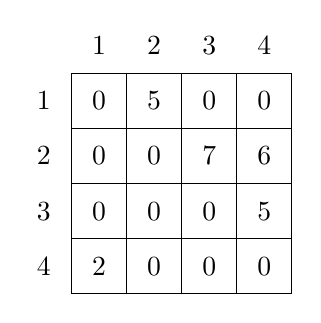
\begin{tikzpicture}[scale=0.7]
\draw (0,0) grid (4,4);
\node at (0.5,0.5) {2};
\node at (1.5,0.5) {0};
\node at (2.5,0.5) {0};
\node at (3.5,0.5) {0};
\node at (0.5,1.5) {0};
\node at (1.5,1.5) {0};
\node at (2.5,1.5) {0};
\node at (3.5,1.5) {5};
\node at (0.5,2.5) {0};
\node at (1.5,2.5) {0};
\node at (2.5,2.5) {7};
\node at (3.5,2.5) {6};
\node at (0.5,3.5) {0};
\node at (1.5,3.5) {5};
\node at (2.5,3.5) {0};
\node at (3.5,3.5) {0};
\node at (-0.5,0.5) {4};
\node at (-0.5,1.5) {3};
\node at (-0.5,2.5) {2};
\node at (-0.5,3.5) {1};
\node at (0.5,4.5) {1};
\node at (1.5,4.5) {2};
\node at (2.5,4.5) {3};
\node at (3.5,4.5) {4};
\end{tikzpicture}
\end{center}
\end{samepage}

Nedostatak prikaza matricom susjedstva
je što matrica sadrži $n^2$ elemenata,
a obično je većina njih nula.
Zbog toga se taj prikaz ne može koristiti
ako je graf velik.

\subsubsection{Prikaz listom bridova}

\index{lista bridova}

\key{Lista bridova} sadrži sve bridove grafa
u nekom redoslijedu.
To je praktičan način prikaza grafa
ako algoritam obrađuje sve bridove grafa
i nije potrebno pronaći bridove koji počinju
u danom čvoru.

Lista bridova može se pohraniti u vektoru
\begin{lstlisting}
vector<pair<int,int>> edges;
\end{lstlisting}
gdje svaki par $(a,b)$ označava da
postoji brid od čvora $a$ do čvora $b$.
Tako se graf

\begin{center}
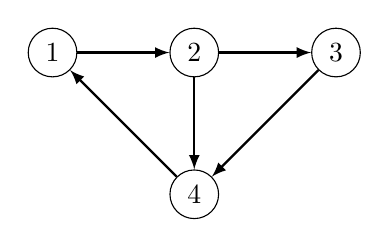
\begin{tikzpicture}[scale=0.9]
\node[draw, circle] (1) at (1,3) {$1$};
\node[draw, circle] (2) at (3,3) {$2$};
\node[draw, circle] (3) at (5,3) {$3$};
\node[draw, circle] (4) at (3,1) {$4$};

\path[draw,thick,->,>=latex] (1) -- (2);
\path[draw,thick,->,>=latex] (2) -- (3);
\path[draw,thick,->,>=latex] (2) -- (4);
\path[draw,thick,->,>=latex] (3) -- (4);
\path[draw,thick,->,>=latex] (4) -- (1);
\end{tikzpicture}
\end{center}
može prikazati na sljedeći način:
\begin{lstlisting}
edges.push_back({1,2});
edges.push_back({2,3});
edges.push_back({2,4});
edges.push_back({3,4});
edges.push_back({4,1});
\end{lstlisting}

\noindent
Ako je graf težinski, struktura se može
proširiti na sljedeći način:
\begin{lstlisting}
vector<tuple<int,int,int>> edges;
\end{lstlisting}
Svaki element ove liste ima
oblik $(a,b,w)$, što znači da
postoji brid od čvora $a$ do čvora $b$ s težinom $w$.
Na primjer, graf

\begin{center}
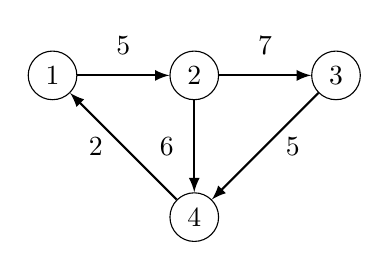
\begin{tikzpicture}[scale=0.9]
\node[draw, circle] (1) at (1,3) {$1$};
\node[draw, circle] (2) at (3,3) {$2$};
\node[draw, circle] (3) at (5,3) {$3$};
\node[draw, circle] (4) at (3,1) {$4$};

\path[draw,thick,->,>=latex] (1) -- node[font=\small,label=above:5] {} (2);
\path[draw,thick,->,>=latex] (2) -- node[font=\small,label=above:7] {} (3);
\path[draw,thick,->,>=latex] (2) -- node[font=\small,label=left:6] {} (4);
\path[draw,thick,->,>=latex] (3) -- node[font=\small,label=right:5] {} (4);
\path[draw,thick,->,>=latex] (4) -- node[font=\small,label=left:2] {} (1);
\end{tikzpicture}
\end{center}
\begin{samepage}
može se prikazati na sljedeći način\footnote{U nekim starijim prevoditeljima (compiler) mora se
koristiti funkcija \texttt{make\_tuple} umjesto vitičastih zagrada (na primjer,
\texttt{make\_tuple(1,2,5)} umjesto \texttt{\{1,2,5\}}).}:
\begin{lstlisting}
edges.push_back({1,2,5});
edges.push_back({2,3,7});
edges.push_back({2,4,6});
edges.push_back({3,4,5});
edges.push_back({4,1,2});
\end{lstlisting}
\end{samepage}
